\documentclass[sigconf]{acmart}

\settopmatter{
  printacmref=false,
  printccs=false,
  printfolios=false
}

\renewcommand\footnotetextcopyrightpermission[1]{}
\pagestyle{plain}

\acmConference{}{}{}
\acmBooktitle{}
\acmPrice{}
\acmDOI{}
\acmISBN{}

\usepackage{graphicx}

\begin{document}

\title{Collecting and Analyzing Multidimensional Data under Local Differential Privacy}

\author{Nabeel Navab}
\affiliation{
\institution{Institute of IT Security, University of Lübeck}
\city{Lübeck}
\country{Germany}
}
\email{nabeel.navab@student.uni-luebeck.de}

\begin{abstract}
The increasing collection of user data by online services and smart devices has raised significant concerns regarding privacy preservation. \textit{Local Differential Privacy}  (LDP) , a privacy model that perturbs data on a user's device before transmission, has emerged as a promising approach for protecting sensitive information while still enabling data analysis. However, applying LDP to multidimensional datasets remains challenging because the utility of collected data often decreases as the number of attributes grows. This paper examines a multidimensional LDP approach that introduces the \textit{Piecewise Mechanism} (PM) and \textit{Hybrid Mechanism} (HM) to improve the accuracy of statistical estimation under strong privacy guarantees. Furthermore, the framework extends LDP techniques to machine learning tasks through privacy-preserving stochastic gradient descent. Experimental results indicate that PM and HM reduce estimation error more effectively than existing multidimensional LDP approaches.




\end{abstract} 
\keywords{
Local Differential Privacy,
Multidimensional Data,
Privacy Preservation,
Statistical Analysis,
Machine Learning
}

\maketitle
\thispagestyle{empty}
\pagestyle{empty}
\markboth{}{}

\section{Introduction}

\textit{Differential Privacy} (DP) protects individual records by limiting the information that can be inferred from published data~\cite{dwork2006}, while LDP applies this protection directly on the user's device before data collection. LDP enables the collection of user data while preserving privacy by perturbing information before it is transmitted to a data collector.
 Although existing LDP mechanisms provide strong privacy guarantees, they are primarily designed for single-dimensional data and often suffer from significant utility degradation when applied to multidimensional datasets. Practical deployments of LDP have also been explored in systems such as RAPPOR~\cite{rappor2014}, which applies randomized response techniques for privacy-preserving data collection.


In practical applications, user records frequently contain multiple numerical and categorical attributes. The framework supports both numerical and categorical attributes, which require different perturbation and estimation strategies under LDP.
 Collecting and analyzing such data under LDP presents a fundamental challenge, as the privacy budget must be distributed across several dimensions, increasing noise and reducing estimation accuracy. Consequently, multidimensional LDP mechanisms must balance local privacy protection against the rapid increase in estimation error caused by perturbing multiple attributes simultaneously.



\section{The Multidimensional LDP Framework}
The multidimensional LDP framework presented in~\cite{wang2019} addresses a key limitation of traditional LDP mechanisms, which often experience substantial utility loss when applied to datasets containing multiple attributes.

 As the dimensionality of the data increases, perturbing every attribute independently introduces excessive noise and reduces the accuracy of statistical analysis.

The framework follows a client-side privacy model in which each user perturbs their data locally before transmission. For multidimensional records, the privacy budget is carefully allocated across attributes to limit utility loss while maintaining the desired privacy guarantees. The perturbed reports are then collected by an aggregator, which reconstructs statistical properties of the original dataset through unbiased estimation techniques. This design enables accurate analysis without requiring access to raw user data.

LDP is formally defined by

\begin{equation}
P[M(x)=y] \leq e^{\epsilon} P[M(x')=y]
\end{equation}

for any two possible inputs $x$ and $x'$ and any output $y$, where $\epsilon$ denotes the privacy budget. Smaller values of $\epsilon$ provide stronger privacy guarantees but typically reduce the utility of the collected data.

A central challenge of multidimensional LDP is the allocation of the privacy budget across multiple attributes. When the available privacy budget is divided among several dimensions, each attribute receives a smaller share of the budget, increasing perturbation noise and reducing estimation accuracy. Consequently, utility decreases as the dimensionality of the dataset grows, motivating the need for specialized multidimensional mechanisms.
The impact of dimensionality on estimation accuracy can be expressed through the variance relationship
\begin{equation}
Var[\hat{\mu}] \propto \frac{d}{n\epsilon^2}
\end{equation}
This relationship illustrates that estimation variance increases with the dimensionality $d$ of the dataset and decreases with the number of users $n$ and the privacy budget $\epsilon$. Consequently, multidimensional datasets become increasingly difficult to analyze accurately under strict privacy constraints, motivating the need for mechanisms such as PM and HM.
The central objective of the framework is to reduce the utility degradation introduced by multidimensional perturbation while preserving rigorous local privacy guarantees.

To address the increase in estimation error caused by perturbing multiple attributes simultaneously, PM applies a piecewise probability distribution that perturbs values within a bounded output range, reducing variance compared to conventional randomized mechanisms. HM combines PM with alternative perturbation strategies and dynamically adapts to different privacy budgets, enabling improved estimation accuracy across high-dimensional datasets.

Unlike traditional LDP approaches that perturb each attribute independently using uniform noise distributions, PM and HM reduce excessive noise accumulation across multiple dimensions. Experimental evaluation shows that both methods achieve lower estimation error than existing multidimensional LDP approaches under varying privacy budgets.



The mechanisms primarily target accurate statistical estimation, enabling aggregate properties such as means and distributions to be reconstructed from privatized reports without revealing individual user records.



\begin{figure}[ht]
\centering
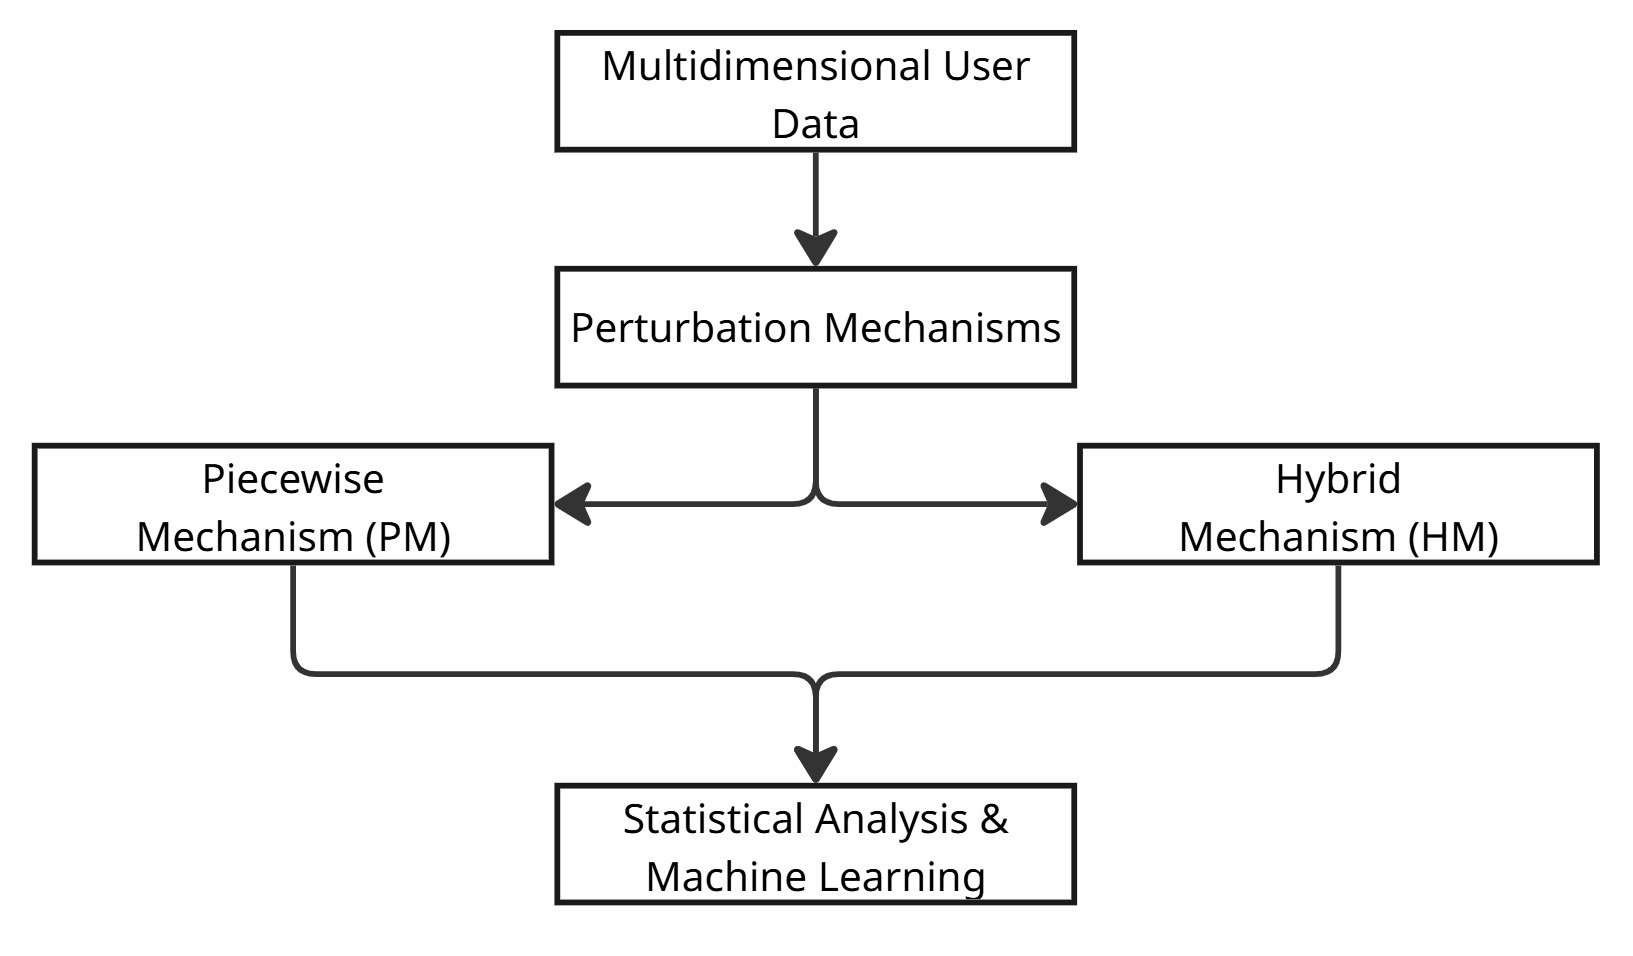
\includegraphics[width=0.9\columnwidth]{framework_workflow.jpg}
\caption{Overview of the multidimensional LDP approach. PM and HM apply local perturbation to enable statistical analysis and machine learning on multidimensional data.}
\label{fig:framework}
\end{figure}

In addition to statistical estimation, the framework supports machine learning applications through privacy-preserving stochastic gradient descent (LDP-SGD). Instead of transmitting raw gradients, users locally perturb their updates before sharing them with the server. This enables model training on sensitive multidimensional data without exposing individual records. The integration of perturbation mechanisms with privacy-preserving stochastic gradient descent enables machine learning on sensitive multidimensional datasets while maintaining formal privacy guarantees.

\section{Experimental Evaluation}

The evaluation compares PM and HM against conventional multidimensional LDP approaches under varying privacy budgets and dimensionalities. Both numerical and multidimensional datasets are considered to investigate how the mechanisms behave as the number of attributes increases. In addition to statistical estimation, the evaluation also examines the applicability of LDP-SGD for privacy-preserving machine learning tasks.

\begin{figure}[h]
\centering
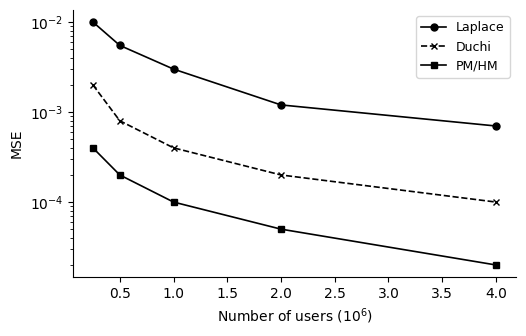
\includegraphics[width=\linewidth]{graph.png}
\caption{Figure 2: Estimation error for PM/HM and conventional LDP approaches under increasing numbers of users. 
 Adapted from~\cite{wang2019}.}

\label{fig:results}
\end{figure}

Figure~\ref{fig:results} illustrates the relationship between the number of users and estimation accuracy for PM/HM and conventional LDP approaches. As the number of users increases, the estimation error decreases across all methods due to the larger amount of aggregated information available for estimation. PM/HM consistently achieve lower error than traditional multidimensional LDP approaches across varying dataset settings.

The evaluation shows that the estimation error increases as dimensionality grows. Compared to conventional approaches that perturb each attribute independently, PM and HM reduce excessive noise accumulation and maintain improved reconstruction accuracy across multiple dimensions.

In addition to aggregate estimation tasks, the experiments examine machine learning using LDP-SGD on perturbed user reports. The results indicate that useful models can still be trained while preserving formal LDP guarantees.







\section{Conclusion}

This paper examined a multidimensional LDP approach for privacy-preserving data collection and analysis. PM and HM reduce estimation error more effectively than conventional LDP approaches while maintaining rigorous local privacy constraints across high-dimensional datasets. In addition, the integration of LDP-SGD demonstrates that useful machine learning models can still be trained on perturbed user reports without exposing individual records.

The evaluation highlights the tradeoff between privacy and analytical accuracy in multidimensional settings and shows that carefully designed perturbation strategies can significantly improve statistical reconstruction under strict privacy budgets.


\bibliographystyle{ACM-Reference-Format}
\bibliography{references}

\end{document}
